\section{Theoretical Aspects of Dendritic Computation}
\label{sec:dendritic_computation_theory}

\begin{figure}
	\centering
	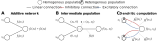
\includegraphics{media/chapters/03_nlif/03_01/nef_multivariate_functions.pdf}%
	{\phantomsubcaption\label{fig:nef_multivariate_functions_a}}%
	{\phantomsubcaption\label{fig:nef_multivariate_functions_b}}%
	{\phantomsubcaption\label{fig:nef_multivariate_functions_c}}%
	\caption[Using dendritic computation to compute multivariate functions in the NEF]{Using dendritic computation to compute multivariate functions in the NEF. \textbf{(A)} Standard NEF networks are additive: summation in activity space corresponds to addition in representation space.
	\textbf{(B)} Computing nonlinear multivariate functions $\phi$ generally requires all variables to be represented in an intermediate population.
	\textbf{(C)} The dendritic computation scheme discussed in here.
	Two pre-populations project onto a post-population with separate excitatory and inhibitory input channels.
	%The nonlinear interaction between these channels is exploited to compute $\phi$.
	}
	\label{fig:nef_multivariate_functions}
\end{figure}

The idea of dendritic computation as pursued here is best explained by exploring how mul\-ti\-va\-ri\-ate functions such as $\phi(x_1, \ldots, x_\ell)$ can be computed in the NEF, and by reviewing some fundamental theoretical properties of neural networks.
Specifically, we analyse three different network architectures (cf.~\Cref{fig:nef_multivariate_functions}).
\enquote{Additive networks} represent the variables $x_1$, $\ldots$, $x_\ell$ in independent neuron populations and cannot approximate most multivariate functions.
In contrast, networks with an intermediate population representing all variables at the same time are universal function approximators.
Dendritic computation relies on non-linear interaction between independent neural input channels.
While not as powerful as networks with an intermediate population, dendritic computation can approximate larger classes of functions well compared to additive networks.

\subsection{Additive Multivariate Networks}
\label{sec:additive_net}

As stated above, our goal is to compute multivariate functions $\phi(x_1, \ldots, x_\ell)$ within the context of the NEF.
%For the sake of simplicity, we mostly discuss bivariate functions of the form $\phi(x_1, x_2)$, but the same considerations apply to more than two input variables as well.
For the sake of simplicity, assume that two pre-populations representing the variables $x_1$, $x_2$ are connected to a common post-population.
To compute $\phi(x_1, x_2)$, we must find connection weights $\vec w_{1, i}$, $\vec w_{2, i}$ such that the following holds for every post-neuron $i$
\begin{align}
	a_i(\phi(x_1, x_2))
		= G_i \bigl[
			\langle \vec e_i, \phi(x_1, x_2) \rangle
		\bigr]
		\supposedEq G_i\bigl[
			\langle \vec w_{1, i}, \vec a^\mathrm{pre}_1(x_1) \rangle + \langle \vec w_{2, i}, \vec a^\mathrm{pre}_2(x_2)
		\rangle\bigr] \,.
	\label{eqn:nef_multivariate_addition}
\end{align}
Here, $a_i$ is the desired post-neuron activity according to the normative tuning-curve constraint (eq.~2.??).
% TODO: Add correct reference
As discussed in the context of the NEF transformation principle in Section~2.3.5, we assume that the current-translation function $J_i$ is part of the individual neuron response curve $G_i$, and that the currents induced by the pre-populations are summed.
% TODO: Add correct reference

Now, consider multivariate functions that can be decomposed into a sum of two univariate functions, i.e., $\phi(x_1, x_2) = f_1(x_1) + f_2(x_2)$ (\Cref{fig:nef_multivariate_functions_a}).
We can easily find weights $\vec w_{1, i}$, $\vec w_{2, i}$ that approximate such a function using the encoder-decoder split of the NEF.
Computing function decoders $\mat D^{f_1}$, $\mat D^{f_2}$ and using the identity $(\vec w_i)^T = \vec e_i \mat D$, we have
\begin{align*}
	G_i\bigl[
	  \langle
	  	\vec e_i \mat D^{f_1},
	  	\vec a^\mathrm{pre}_1(x_1)
	  \rangle
	+ \langle
	  	\vec e_i \mat D^{f_2},
		\vec a^\mathrm{pre}_2(x_2)
	\rangle\bigr] = 
	G_i\bigl[\langle \vec e_i, \mat D^{f_1} \vec a_1^\mathrm{pre}(x_1) + \mat D^{f_2} \vec a_2^\mathrm{pre}(x_2) \rangle\bigr]
	\approx a_i\bigl(f_1(x_1) + f_2(x_2)\bigr) \,.
\end{align*}
This equation can be interpreted as saying that addition in activity space (i.e., summing weighted pre-activities, eq.~\ref{eqn:nef_multivariate_addition}) is equal to addition in represented space.
In other words, standard NEF networks are \emph{additive}.
%\footnote{We already used the additivity of NEF networks in~Section~2.3.5, when we discussed the dynamics principle.}
Summing functions incurs no additional decoding error.

\begin{figure}
	\centering
	\includegraphics{media/chapters/03_nlif/03_01/perceptron.pdf}%
	{\phantomsubcaption\label{fig:perceptron_a}}%
	{\phantomsubcaption\label{fig:perceptron_b}}%
	\caption[Additive networks are a generalisation of the perceptron]{Additive networks are a generalisation of the perceptron. \textbf{(A)} An additive network is a sum of arbitrary univariate functions. \textbf{(B)} A perceptron is an additive network with functions of the form $f_i(x_i) = w_i x_i + \beta \ell^{-1}$. The weights $w_i$ are learned such that the output approximates a desired function.}
\end{figure}

\subsubsection{Additive networks cannot compute most multivariate functions}
The only way to compute general multivariate functions $\phi(x_1, x_2)$ in additive networks is to \emph{approximate} $\phi$ as an additive univariate decomposition.
As expressed by the following theorem (see Appendix~B.3.1 for a proof), it is \emph{impossible} to compute many continuous multi-variate $\phi$ using such additive networks.%
\footnote{We limit Theorem~\ref{thm:xor_general} to continuous functions for the sake of simplicity.
However, we conjecture that the same results hold for larger classes of functions, for example square Lebesgue integrable functions.}
This is true even if we can decode arbitrary univariate functions $f_1$, $\ldots$, $f_\ell$ over the pre-variables (this is equivalent to having an infinite number of pre-neurons, see below), and we were able to freely choose a fixed nonlinearity $\sigma$ (cf.~\Cref{fig:perceptron_a}).

\begin{theorem}
\label{thm:xor_general}
Let $\ell > 1$, $\Xrepr \subset \mathbb{R}^\ell$ and $\mathbb{Y} \subset \mathbb{R}$ be compact sets, and $\sigma$, $\phi$, $f_i$ be continuous.
For any fixed $\sigma : \mathbb{R} \longrightarrow \mathbb{Y}$, there always exist $\phi : \Xrepr \longrightarrow \mathbb{Y}$ such that there are no $f_1$, $\ldots$, $f_\ell : \mathbb{R}  \longrightarrow \mathbb{R}$ with the property
$\phi(x_1, \ldots, x_\ell) = \sigma(\xi) = \sigma\bigl( f_1(x_1) + \ldots + f_\ell(x_\ell) \bigr)$ for all $(x_1, \ldots, x_\ell) \in \Xrepr$.
\end{theorem}

\begin{figure}
	\centering
	\includegraphics{media/chapters/03_nlif/03_01/xor_visualisation.pdf}%
	{\phantomsubcaption\label{fig:xor_visualisation_a}}%
	{\phantomsubcaption\label{fig:xor_visualisation_b}}%
	{\phantomsubcaption\label{fig:xor_visualisation_c}}%
	{\phantomsubcaption\label{fig:xor_visualisation_d}}%
	{\phantomsubcaption\label{fig:xor_visualisation_e}}%
	\caption[Visualisation of the XOR decision problem for different classifiers]{Visualisation of the XOR decision problem for different classifiers. The goal is to find classifier parameters such that the four samples are classified as depicted.
	The background corresponds to the sign of the monotonic function $\sigma(\xi)$.
	\textbf{(A)} The linear decision boundary formed by the Perceptron cannot solve the XOR problem.
	\textbf{(B)} This holds for any function of the form $\sigma(f_1(x_1) + f_2(x_2))$, here $f_1(x_1) = \cos(2\pi x_1)$ and $f_2(x_2) = \sin(2\pi x_2)$.
	\textbf{(C)} A multi-layer Perceptron (MLP) of the form $\sum_i w_i \sigma(e_i^1 x_1 + e_i^2 x_2 + \beta_i )$ can solve the problem, although the decision boundary is quite erratic.
	\textbf{(D)} An alternative solution using the nonlinearity $\sigma'(\xi) = \sigma(\xi^2 - 1)$.
	\textbf{(E)} Multiplication of two real-valued variables $x_1$, $x_2$ can be seen as a continuous form of the XOR problem.
	Additive networks cannot compute this function.
	}
	\label{fig:xor_visualisation}
\end{figure}

\subsubsection{The Perceptron and XOR}
Consider monotonic $\sigma$ and affine $f_i$ of the form $w_i x_i + \beta \ell^{-1}$.
We obtain the \emph{perceptron}, an early single-layer neural network (cf.~\Cref{fig:perceptron_b}; \cite{rosenblatt1958perceptron}).
\Citet[Chapter~2; originally published in 1969]{minsky1987perceptrons} point out that such networks cannot compute the boolean XOR function (\Cref{fig:xor_visualisation_a}).%
\footnote{\Citet{minsky1987perceptrons} note that the perceptron was proved by Rosenblatt to \enquote{learn to do anything it was possible to program it to do}; this ambiguous statement endowed researchers with a surplus of optimism---especially since perceptrons could sometimes learn to solve difficult problems.
Among other factors, realising that these networks could not be \emph{programmed} to solve a simple problem such as XOR led to what some call \enquote{the first AI winter} \citep[e.g.,][]{muthukrishnan2020brief}.}
%In the continuous domain, the same is true for multiplication over $\mathbb{X} = [-1, 1]^2$, that is $\phi(x_1, x_2) = x_1 x_2$ (\Cref{fig:xor_visualisation_a}).
Even the general additive networks from our theorem cannot solve a \emph{weaker} version of the XOR problem, formalised below.

\begin{definition}
\label{def:weak_xor}
A function $\phi(x, y)$ solves the \emph{weak XOR problem} if there exist $a_0, b_0, a_1, b_1$ with
\begin{align*}
	\big( \phi(a_0, b_0) < \phi(a_0, b_1) \big) \wedge
	\big( \phi(a_1, b_1) < \phi(a_0, b_1) \big) \wedge
	\big( \phi(a_0, b_0) < \phi(a_1, b_0) \big) \wedge
	\big( \phi(a_1, b_1) < \phi(a_1, b_0) \big) \,.
\end{align*}
\end{definition}
That is, we merely require $\phi(a_0, b_0)$ and $\phi(a_1, b_1)$ to be larger than $\phi(a_0, b_1)$ and $\phi(b_1, b_0)$.

\begin{restatable}{theorem}{ThmWeakXor}
\label{thm:weak_xor}
Let $\sigma$ be monotonic. Then, an additive network of the form $\phi(x_1, x_2) = \sigma(f_1(x_1) + f_2(x_2))$ cannot solve the weak XOR problem.
\end{restatable}
This may be surprising, given that, as depicted in \Cref{fig:xor_visualisation_b}, we can generate highly nonlinear classification boundaries.
We provide a proof in Appendix~B.3.2.

To solve the XOR problem, we can either, as discussed next, use multi-layer networks (cf.~\Cref{fig:xor_visualisation_c}), or, alternatively make $\sigma$ non-monotonic.
As depicted in \Cref{fig:xor_visualisation_d}, setting $\sigma(\xi) = \xi^2 - 1$ allows us to solve the XOR problem.
This illustrates our goal with dendritic computation: exploit \enquote{more powerful} $\sigma$ to approximate a larger class of functions.

Still, the functions that we can compute using additive networks are limited, even if we can freely choose $\sigma$.
For example, we can compute $x_1 x_2$ for $(x_1, x_2) \in [\epsilon, 1]^2$ and $0 < \epsilon < 1$ by setting $f_1$ and $f_2$ to the logarithm and $\sigma$ to the exponential.
However, it is impossible to find functions that compute multiplication over all four quadrants---which can be seen as a continuous version of the XOR problem (\Cref{fig:xor_visualisation_e}).
More precisely, allowing $x_1$, $x_2$ to be zero makes it impossible to compute multiplication in these networks (proof in Appendix~B.3.3).
\begin{restatable}{theorem}{ThmMultiplication}
\label{thm:multiplication}
There are no continuous, real-valued functions $f_1$, $f_2$, $\sigma$ such that $\sigma(f_1(x_1) + f_2(x_2)) = x_1 x_2$ for all $(x_1, x_2) \in [0, 1]^2$.
\end{restatable}


%Choosing this $\sigma$ implicitly introduces a non-linear interaction between the variables $x_1$, $x_2$, for example
%\begin{align*}
%	\sigma\left( (w_1 x_1 + w_2 x_2 + \beta)^2 - 1\right) = 
%	\sigma\left( w_1^2 x_1^2 + w_2^2 x_2^2 + 2 w_1 w_2 x_1 x_2 + 2 w_1 \beta x_1 + 2 w_2 \beta x_2 + \beta^2  - 1\right) \,.
%\end{align*}
%The product-term $w_1 w_2 x_1 x_2$ can be exploited to %compute multiplication-like functions.
%Still, as stated in Theorem~1, there inevitably is a large set of functions that we cannot compute.
% TODO Add reference

\subsection{Multi-Layer Networks}

\begin{figure}
	\includegraphics{media/chapters/03_nlif/03_01/mlp.pdf}
	\caption[Sketch of a two-layer neural network]{Sketch of a two-layer neural network with rectified linear units (ReLUs). If the encoding vectors $\vec e_i$ and the biases $\beta_i$ are sampled appropriately, this network is a universal function approximator.}
	\label{fig:mlp}
\end{figure}

As already mentioned in Section~2.3.5, an individual NEF population can be interpreted as a two-layer neural network (cf.~\Cref{fig:mlp}).
% TODO: Add reference
As long as the encoding vectors are sampled from $\ell$-dimensional hypersphere and $x$-intercepts are uniformly distributed, such a neuron population is a universal function approximator.
The following theorem states this more formally for neurons with a rectified linear unit (ReLU) nonlinearity, i.e., $\sigma(\xi) = \max\{0, \xi\}$.

\begin{theorem}
\label{thm:two_layer_universal}
Let $\ell \geq 1$, and $\phi : \mathbb{B}^\ell \longrightarrow \mathbb{R}$ be a continuous function mapping from the $\ell$-dimensional unit ball onto $\mathbb{R}$.
Furthermore, let $\sigma(\xi) = \max\{0, \xi\}$, $\vec e_i$ be sampled uniformly from the unit-sphere $\mathbb{S}^\ell$, and $\beta_i$ be sampled uniformly from $[-1, 1]$.
There exist $d_i \in \mathbb{R}$ such that
\begin{align}
	\phi(\vec x) = \lim_{\Npop \to \infty} \sum_{i = 1}^{\Npop} d_i \sigma\bigl( \langle \vec e_i, \vec x \rangle + \beta_i \bigr) \quad \text{for all} \quad \vec x \in \mathbb{B}^\ell \,.
	\label{eqn:two_layer_network}
\end{align}
\end{theorem}

This follows from \citet{hornik1989multilayer}.
We provide a sketch of a proof in Appendix~B.3.3.
This theorem can be easily extended to hold for arbitrary compact domains $\Xrepr$, codomain dimensionalities, and other neural nonlinearities $\sigma$.

%It may not be obvious why \cref{eqn:two_layer_network} describes a \enquote{two-layer} neural network.
%In essence, the encoding weights $\vec e_i$ map $\vec x$ onto the input of one of the $N$ neurons with nonlinearity $\sigma$.
%This step forms the \enquote{first} or \enquote{hidden layer}.
%The decoding weights $d_i$ then map the neural activities $\sigma(\xi_i)$ onto the output, which forms the \enquote{second layer} (cf.~Figure~2.20).
%% TODO: Add actual reference

\subsubsection{The role of uniformly sampled encoders}
Theorem~\ref{thm:two_layer_universal} requires that the encoding vectors $\vec e_i$ are uniformly sampled from the hypersphere $\mathbb{S}^\ell$.%
\footnote{As follows from the proof of Theorem~\ref{thm:two_layer_universal} in Appendix~B.3.3, there technically are weaker requirements for this.
One example is given in \citet{gosmann2015precise}; given a specific function $\phi$ (such as multiplication), there are certain distributions of encoding vectors that minimise the decoding error.
In fact, global optimisation methods such as stochastic gradient descent can be seen as systematically selecting such \enquote{optimal} encoders.}
To get an intuition as for why this is important, consider the case where the $\vec e_i$ are axis-aligned, i.e., $\|\vec e_i\|_0 = 1$ (cf.~Appendix~A.1).
% TODO: Add reference for zero-norm in Appendix~A.1
In this case, we can split \cref{eqn:two_layer_network} into $\ell$ sub-networks, each decoding a function over a single variable $x_\ell$
\begin{align*}
		\sum_{i = 1}^N d_i \sigma\bigl( \langle \vec e_i, \vec x \rangle - \beta_i \bigr)
	= 	\sum_{j = 1}^\ell \sum_{i = 1}^{N_j} d_{j i} \sigma\bigl( e_{j i} x_j - \beta_{j i} \bigr) \,, \text{where } e_{j i} \in \{ -1, 1\} \,.
\end{align*}
This is equivalent to the additive networks we discussed before.
We can only decode sums of univariate functions over the individual $x_j$ from the pre-population.

\subsubsection{Intermediate populations}
%We now know that we can indeed approximate multivariate functions in the NEF with an arbitrarily small error.
%The pre-condition for this is that all variables over which we would like to compute a $\phi$ represented in the same neuron population with non-axis aligned encoding vectors $\vec e_i$.
As discussed by \citep[Chapter~6]{eliasmith2003neural}, we need to introduce intermediate populations if, as an example, variables $x_1$, $x_2$ are represented in independent pre-populations, and we would like to compute a multivariate function $\phi(x_1, x_2)$.
This intermediate population represents a vectorial quantity $\vec z = (x_1, x_2)$ (cf.~\Cref{fig:nef_multivariate_functions_b}).
This can be accomplished by computing the univariate functions $f_1(x_1) = (x_1, 0)$ and $f_2(x_2) = (0, x_2)$ in the connections to the intermediate population.
According to Theorem~\ref{thm:two_layer_universal} we can then decode any multivariate function from the intermediate population.

\subsubsection{Potential issues with intermediate populations}
In theory, the number of neurons required to cover a $d$-dimensional space is exponential in $d$.
Representing a $d$-dimensional quantity in an intermediate population thus requires many neurons to achieve a certain decoding error.
In practice, it is quite difficult to judge the number of neurons required to decode a certain function $f$ a-priori; the decoding error heavily depends on $f$ and the encoding vectors $\vec e_i$.

Another problem arises when modelling neurobiological systems.
There may be no indication that an intermediate population exists in a particular biological circuit, but the function can be modelled well as a multivariate function.
An example of this would be the aforementioned attention system, where a group of control neurons modulates another population without an intermediary \citep{bobier2014unifying}.

Finally, there is the issue of noise.
In spiking neural networks, every intermediate neuron population introduces additional noise due to static distortion and spike noise \citep[Section~2.2.2]{eliasmith2003neural}.
We see the effects of this later.

\subsection{Dendritic Computation}
\label{sec:dendritic_computation_theory_dendritic}

Dendritic computation is one way to partially alleviate the limitations arising from intermediate populations.
The basic idea is that each neuron possesses $k$ \emph{input channels}.
Input fed through these channels interacts nonlinearly, modelling information processing within the dendrites.

\begin{figure}
	\includegraphics{media/chapters/03_nlif/03_01/dendritic_computation.pdf}%
	{\phantomsubcaption\label{fig:dendritic_computation_net}}%
	{\phantomsubcaption\label{fig:dendritic_computation_fun}}%
	\caption[Overview of our notion of dendritic computation.]{Overview of our notion of dendritic computation. \textbf{(A)} Neuron with an excitatory and inhibitory input channel. In a network context, these functions are decoded from pre-populations representing these variables. Connectivity can be constrained such that excitatory and inhibitory pre-neurons only connect to the corresponding channel. \textbf{(B)} Conceptually, each channel receives a sum of univariate functions computed over the pre-variables $x_1$, $\ldots$, $x_\ell$.}
\end{figure}

Mathematically, the response curve describing the average neural activity is now a multivariate function $\mathscr{G}[\xi_1, \ldots, \xi_k]$, where the $\xi_i$ are linear combinations of the pre-activities (\Cref{fig:dendritic_computation_net}).
To compute $\phi(x_1, \ldots, x_\ell)$, the following must hold for each post-neuron $i$
\begin{align}
	\begin{aligned}
	a_i\bigl(\phi(x_1, \ldots, x_\ell)\bigr) &\supposedEq
	\mathscr{G} \bigl[
		\langle \vec w_{1, i}^1, \vec a^\mathrm{pre}_1(x_1) \rangle + \ldots +
		\langle \vec w_{\ell, i}^1, \vec a^\mathrm{pre}_\ell(x_\ell) \rangle, \ldots,\\
%	&~\quad\quad\vdots, \\
	&~\hspace{1.66em}
		\langle \vec w_{1, i}^k, \vec a^\mathrm{pre}_1(x_1) \rangle + \ldots +
		\langle \vec w_{\ell, i}^k, \vec a^\mathrm{pre}_\ell(x_\ell) \rangle
	\bigr]
	\end{aligned}
	\label{eqn:dendritic}
\end{align}
where $a_i(\phi(x_1, \ldots, x_\ell))$ expresses the normative tuning constraint defined in Section~2.3.2.
% TODO: Add correct reference

Note that we deliberately left the concept of an \enquote{input channel} a little vague.
An input channel could either refer to a different location in the dendritic tree, different synapse types (e.g., excitatory or inhibitory synapses), or even the effects of signalling molecules such as hormones.
We discuss examples of model neurons with multiple input channels in \Cref{sec:nlif}.

\subsubsection{Mathematical analysis}
More formally, using $\sigma(\xi_1, \ldots, \xi_\ell)$ as an abstract nonlinearity and assuming that we can compute any univariate function $g_i^j$ over $\xi_1, \ldots, \xi_\ell$, we have (\Cref{fig:dendritic_computation_fun})
\begin{align}
	\sigma \bigl(
		g_{1}^1(x_1) + \ldots + g_{\ell}^1(x_\ell), \ldots, g_{1}^k(x_1) + \ldots + g_{\ell}^k(x_\ell)
	\bigr) = \phi(x_1, \ldots, x_\ell) \,.
	\label{eqn:dendritic_computation_theory}
\end{align}
Such networks are more powerful than additive networks.
For example, let $\sigma(\xi_1, \xi_2) = \xi_1 \xi_2$.
Now, if we set the functions feeding into the second channel to one, i.e., $g_{1, i}^2(x_1) = \ldots = g_{\ell, 1}^2(x_\ell) = 1$, we obtain an additive network.
Of course, using the same $\sigma$, we can, in contrast to additive networks, compute products of the pre-variables over arbitrary domains.

Still, independent of $\sigma$, and similarly to additive networks, dendritic computation networks are not universal function approximators (see Appendix~B.3.5~for the theorem and proof).

%\begin{theorem}
%\label{thm:dendritic_compuation_incomplete}
%Let $\ell > 1$, $\Xrepr \subset \mathbb{R}^\ell$ and $\mathbb{Y} \subset \mathbb{R}$ be compact sets, and $\sigma$, $\phi$, $g^j_i$ be continuous.
%For any fixed $\sigma : \mathbb{R}^k \longrightarrow \mathbb{Y}$, there always exist $\phi : \Xrepr \longrightarrow \mathbb{Y}$ such that there are no $g^1_1$, $\ldots$, $g^k_\ell : \mathbb{R}  \longrightarrow \mathbb{R}$ with the property
%$\phi(x_1, \ldots, x_\ell) = \sigma(\xi_1, \ldots, \xi_k) = \sigma\bigl( g^1_1(x_1) + \ldots + g^1_\ell(x_\ell), \ldots,  g^k_1(x_1) + \ldots + g^k_\ell(x_\ell)\bigr)$ for all $(x_1, \ldots, x_\ell) \in \Xrepr$.
%\end{theorem}

%\subsubsection{Interaction between excitation and inhibition}
%\Cref{fig:nef_multivariate_functions_c} shows an example of a neural network exploiting nonlinear interactions between excitatory and inhibitory synapses.
%Assume that each neuron in the post population possesses an independent excitatory and inhibitory channel, and that the two pre-population represent $x_1$, $x_2$, respectively, and project onto both channels.
%The activity of a single post-neuron $i$ is hence given as
%\begin{align*}
%	\mathscr{G}_i\bigl[
%		\langle
%			\vec w^1_\mathrm{E},
%			\vec a_\mathrm{pre}^1(\vec x_1)
%		\rangle + \langle
%			\vec w^2_\mathrm{E},
%			\vec a_\mathrm{pre}^2(\vec x_2)
%		\rangle,
%		\langle
%			\vec w^1_\mathrm{I},
%			\vec a_\mathrm{pre}^1(\vec x_1)
%		\rangle + \langle
%			\vec w^2_\mathrm{I},
%			\vec a_\mathrm{pre}^2(\vec x_2)
%		\rangle
%	\bigr] \,,
%\end{align*}
%where $\vec w_\mathrm{I}$ and $\vec w_\mathrm{E}$ are the excitatory and inhibitory synaptic weights, and $\vec a_\mathrm{pre}$ are the activities of the pre-populations.
%Assuming that we can decode arbitrary univariate functions over $x_1$, $x_2$ from the pre-populations, our goal is to find functions $g_\mathrm{E}^1(x_1)$, $g_\mathrm{E}^2(x_2)$, $g_\mathrm{I}^1(x_1)$, $g_\mathrm{I}^2(x_2)$, such that the total activity of our neuron has some desired value, i.e.,
%\begin{align*}
%	a_i^\mathrm{post}(\phi(x_1, x_2)) \supposedEq \mathscr{G}_i\bigl[
%		g_\mathrm{E}^1(x_1) + g_\mathrm{E}^2(x_2),
%		g_\mathrm{I}^1(x_1) + g_\mathrm{I}^2(x_2)
%	\bigr] \,.
%\end{align*}


\subsection{Numerical Exploration}
\label{sec:dendritic_computation_theory_numerical}

The above considerations are quite theoretical and provide only limited insight into the practical impact of choosing one network type over the other.
In this section, we discuss a simple numerical experiment that highlights the function approximation errors obtained with different network types for functions $\phi$ of varying \enquote{complexity}.
We use experiments similar to the following throughout this chapter to characterise different network- and neuron-types.

\begin{figure}
	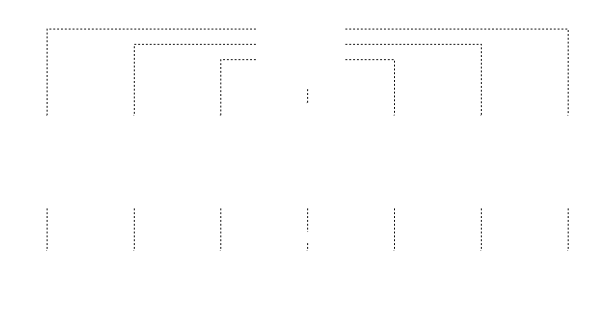
\includegraphics{media/chapters/03_nlif/03_01/2d_functions_overview_overlay.pdf}%
	\kern-157.24mm\includegraphics{media/chapters/03_nlif/03_01/2d_functions_overview.pdf}
	\caption[Overview of our procedure for generating random 2D functions]{Overview of our procedure for generating random 2D functions. \textbf{(A)} We sample a 2D array from a normal distribution (size of the array depends on the filter width; negative values in red, positive in blue). \textbf{(B)} The noise is filtered by convolving with a Gaussian kernel with standard-deviation $\sigma$ (for large filter widths, i.e., small $\sigma^{-1}$, only a small portion of the filter is depicted). \textbf{(C)} The resulting functions are transformed to have mean zero (i.e., no DC component) and a standard deviation of one.}
	\label{fig:2d_functions_overview}
\end{figure}

To analyse different network architectures, w
e randomly generate two-dimensional functions $\phi(x_1, x_2)$ from band-limited white noise with standard deviation one and mean zero.
The band-limit is enforced by filtering with a Gaussian filter kernel with standard deviation $\sigma$.
This is depicted in \Cref{fig:2d_functions_overview}.
Large $\sigma$ result in functions with no high frequencies; such functions are approximately linear.
In contrast, small $\sigma$ result in quite intricate random structures.
Correspondingly, $\sigma^{-1}$ can be seen as a proxy for the \enquote{complexity} of a function.
Small $\sigma^{-1}$ result in low-complexity functions, large $\sigma^{-1}$ in high-complexity functions.
